\documentclass[1p]{elsarticle_modified}
%\bibliographystyle{elsarticle-num}

%\usepackage[colorlinks]{hyperref}
%\usepackage{abbrmath_seonhwa} %\Abb, \Ascr, \Acal ,\Abf, \Afrak
\usepackage{amsfonts}
\usepackage{amssymb}
\usepackage{amsmath}
\usepackage{amsthm}
\usepackage{scalefnt}
\usepackage{amsbsy}
\usepackage{kotex}
\usepackage{caption}
\usepackage{subfig}
\usepackage{color}
\usepackage{graphicx}
\usepackage{xcolor} %% white, black, red, green, blue, cyan, magenta, yellow
\usepackage{float}
\usepackage{setspace}
\usepackage{hyperref}

\usepackage{tikz}
\usetikzlibrary{arrows}

\usepackage{multirow}
\usepackage{array} % fixed length table
\usepackage{hhline}

%%%%%%%%%%%%%%%%%%%%%
\makeatletter
\renewcommand*\env@matrix[1][\arraystretch]{%
	\edef\arraystretch{#1}%
	\hskip -\arraycolsep
	\let\@ifnextchar\new@ifnextchar
	\array{*\c@MaxMatrixCols c}}
\makeatother %https://tex.stackexchange.com/questions/14071/how-can-i-increase-the-line-spacing-in-a-matrix
%%%%%%%%%%%%%%%

\usepackage[normalem]{ulem}

\newcommand{\msout}[1]{\ifmmode\text{\sout{\ensuremath{#1}}}\else\sout{#1}\fi}
%SOURCE: \msout is \stkout macro in https://tex.stackexchange.com/questions/20609/strikeout-in-math-mode

\newcommand{\cancel}[1]{
	\ifmmode
	{\color{red}\msout{#1}}
	\else
	{\color{red}\sout{#1}}
	\fi
}

\newcommand{\add}[1]{
	{\color{blue}\uwave{#1}}
}

\newcommand{\replace}[2]{
	\ifmmode
	{\color{red}\msout{#1}}{\color{blue}\uwave{#2}}
	\else
	{\color{red}\sout{#1}}{\color{blue}\uwave{#2}}
	\fi
}

\newcommand{\Sol}{\mathcal{S}} %segment
\newcommand{\D}{D} %diagram
\newcommand{\A}{\mathcal{A}} %arc


%%%%%%%%%%%%%%%%%%%%%%%%%%%%%5 test

\def\sl{\operatorname{\textup{SL}}(2,\Cbb)}
\def\psl{\operatorname{\textup{PSL}}(2,\Cbb)}
\def\quan{\mkern 1mu \triangleright \mkern 1mu}

\theoremstyle{definition}
\newtheorem{thm}{Theorem}[section]
\newtheorem{prop}[thm]{Proposition}
\newtheorem{lem}[thm]{Lemma}
\newtheorem{ques}[thm]{Question}
\newtheorem{cor}[thm]{Corollary}
\newtheorem{defn}[thm]{Definition}
\newtheorem{exam}[thm]{Example}
\newtheorem{rmk}[thm]{Remark}
\newtheorem{alg}[thm]{Algorithm}

\newcommand{\I}{\sqrt{-1}}
\begin{document}

%\begin{frontmatter}
%
%\title{Boundary parabolic representations of knots up to 8 crossings}
%
%%% Group authors per affiliation:
%\author{Yunhi Cho} 
%\address{Department of Mathematics, University of Seoul, Seoul, Korea}
%\ead{yhcho@uos.ac.kr}
%
%
%\author{Seonhwa Kim} %\fnref{s_kim}}
%\address{Center for Geometry and Physics, Institute for Basic Science, Pohang, 37673, Korea}
%\ead{ryeona17@ibs.re.kr}
%
%\author{Hyuk Kim}
%\address{Department of Mathematical Sciences, Seoul National University, Seoul 08826, Korea}
%\ead{hyukkim@snu.ac.kr}
%
%\author{Seokbeom Yoon}
%\address{Department of Mathematical Sciences, Seoul National University, Seoul, 08826,  Korea}
%\ead{sbyoon15@snu.ac.kr}
%
%\begin{abstract}
%We find all boundary parabolic representation of knots up to 8 crossings.
%
%\end{abstract}
%\begin{keyword}
%    \MSC[2010] 57M25 
%\end{keyword}
%
%\end{frontmatter}

%\linenumbers
%\tableofcontents
%
\newcommand\colored[1]{\textcolor{white}{\rule[-0.35ex]{0.8em}{1.4ex}}\kern-0.8em\color{red} #1}%
%\newcommand\colored[1]{\textcolor{white}{ #1}\kern-2.17ex	\textcolor{white}{ #1}\kern-1.81ex	\textcolor{white}{ #1}\kern-2.15ex\color{red}#1	}

{\Large $\underline{11n_{90}~(K11n_{90})}$}

\setlength{\tabcolsep}{10pt}
\renewcommand{\arraystretch}{1.6}
\vspace{1cm}\begin{tabular}{m{100pt}>{\centering\arraybackslash}m{274pt}}
\multirow{5}{120pt}{
	\centering
	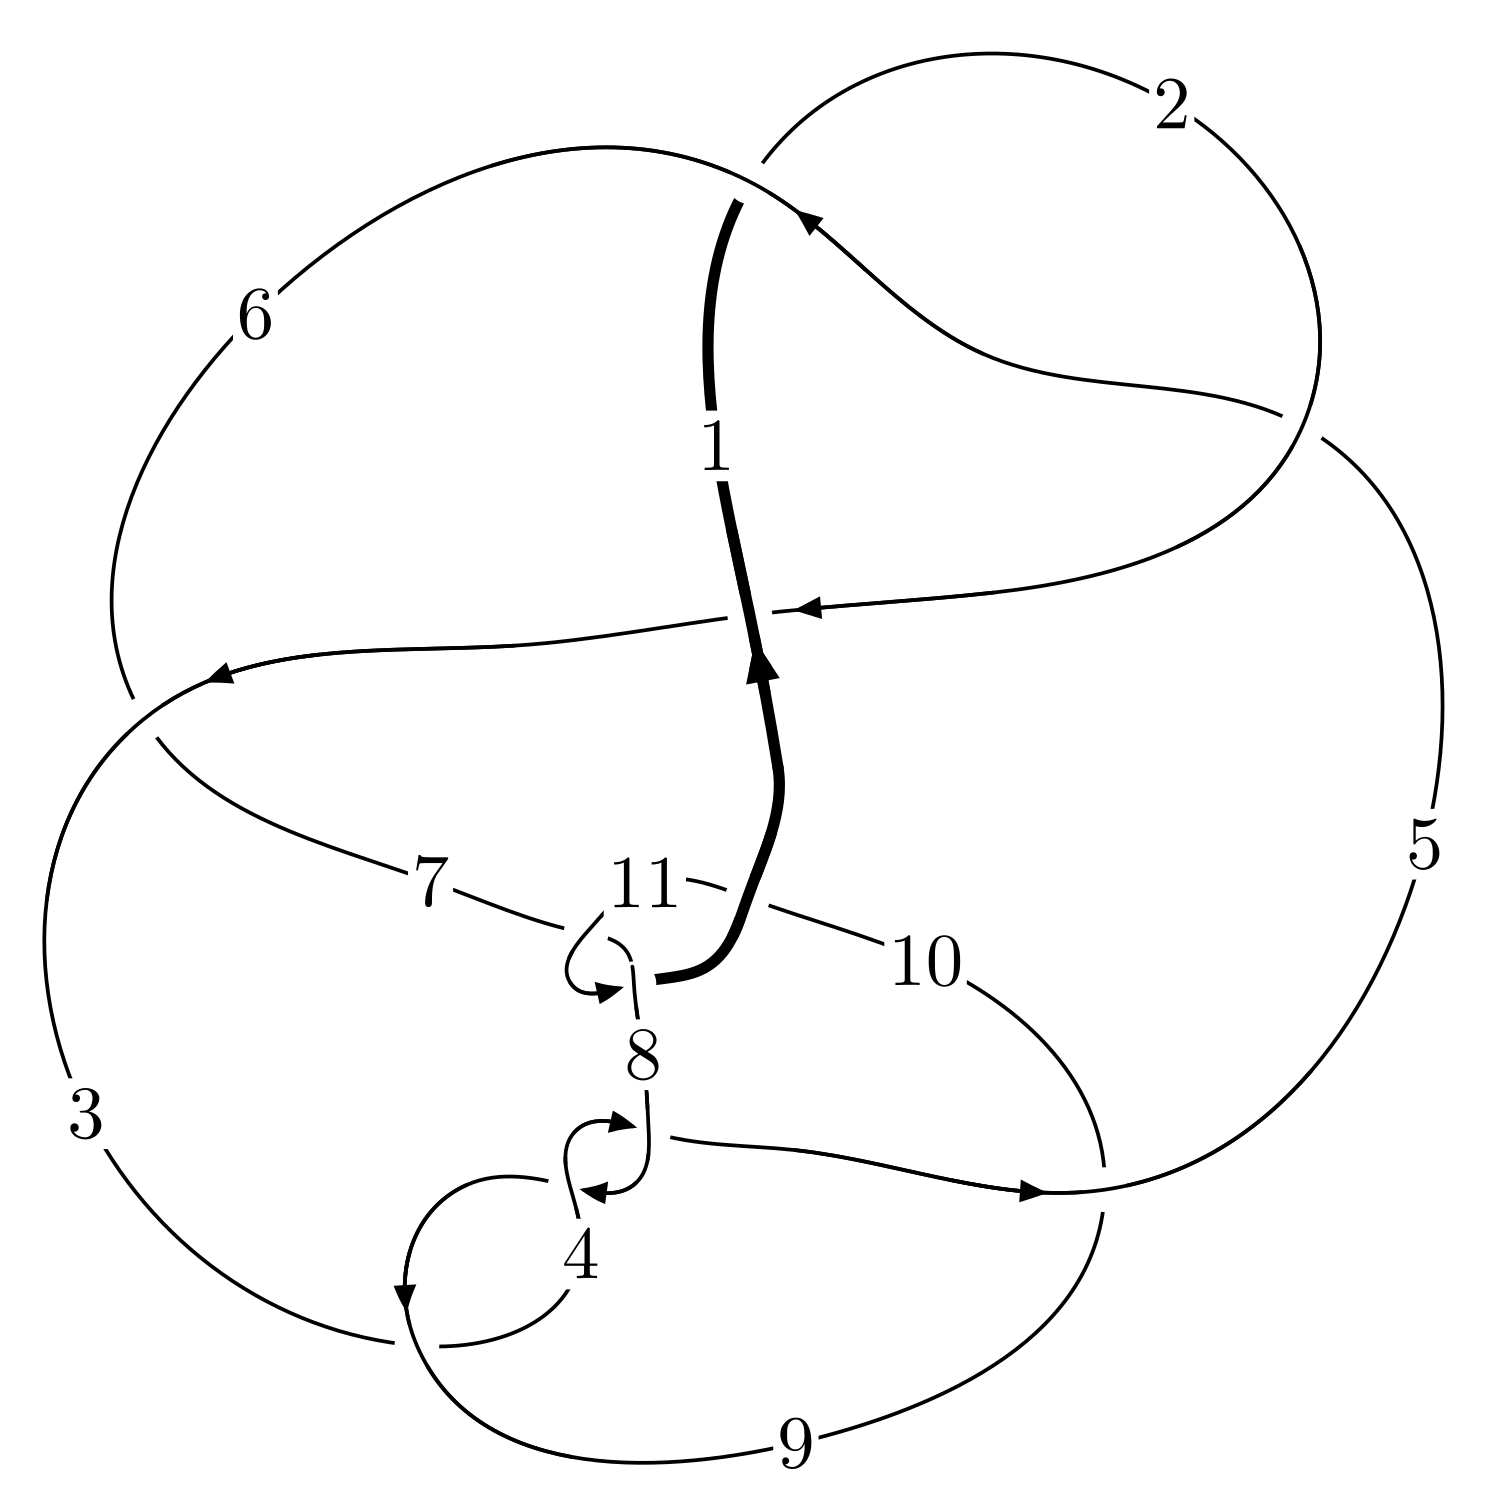
\includegraphics[width=112pt]{../../../GIT/diagram.site/Diagrams/png/706_11n_90.png}\\
\ \ \ A knot diagram\footnotemark}&
\allowdisplaybreaks
\textbf{Linearized knot diagam} \\
\cline{2-2}
 &
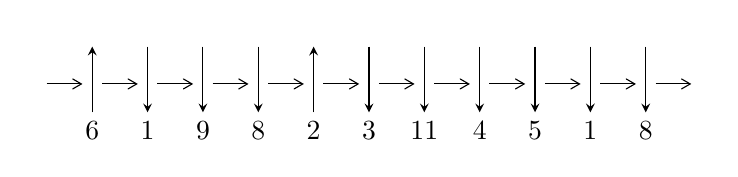
\begin{tikzpicture}[x=20pt, y=17pt]
	% nodes
	\node (C0) at (0, 0) {};
	\node (C1) at (1, 0) {};
	\node (C1U) at (1, +1) {};
	\node (C1D) at (1, -1) {6};

	\node (C2) at (2, 0) {};
	\node (C2U) at (2, +1) {};
	\node (C2D) at (2, -1) {1};

	\node (C3) at (3, 0) {};
	\node (C3U) at (3, +1) {};
	\node (C3D) at (3, -1) {9};

	\node (C4) at (4, 0) {};
	\node (C4U) at (4, +1) {};
	\node (C4D) at (4, -1) {8};

	\node (C5) at (5, 0) {};
	\node (C5U) at (5, +1) {};
	\node (C5D) at (5, -1) {2};

	\node (C6) at (6, 0) {};
	\node (C6U) at (6, +1) {};
	\node (C6D) at (6, -1) {3};

	\node (C7) at (7, 0) {};
	\node (C7U) at (7, +1) {};
	\node (C7D) at (7, -1) {11};

	\node (C8) at (8, 0) {};
	\node (C8U) at (8, +1) {};
	\node (C8D) at (8, -1) {4};

	\node (C9) at (9, 0) {};
	\node (C9U) at (9, +1) {};
	\node (C9D) at (9, -1) {5};

	\node (C10) at (10, 0) {};
	\node (C10U) at (10, +1) {};
	\node (C10D) at (10, -1) {1};

	\node (C11) at (11, 0) {};
	\node (C11U) at (11, +1) {};
	\node (C11D) at (11, -1) {8};
	\node (C12) at (12, 0) {};

	% arrows
	\draw[->,>={angle 60}]
	(C0) edge (C1) (C1) edge (C2) (C2) edge (C3) (C3) edge (C4) (C4) edge (C5) (C5) edge (C6) (C6) edge (C7) (C7) edge (C8) (C8) edge (C9) (C9) edge (C10) (C10) edge (C11) (C11) edge (C12) ;	\draw[->,>=stealth]
	(C1D) edge (C1U) (C2U) edge (C2D) (C3U) edge (C3D) (C4U) edge (C4D) (C5D) edge (C5U) (C6U) edge (C6D) (C7U) edge (C7D) (C8U) edge (C8D) (C9U) edge (C9D) (C10U) edge (C10D) (C11U) edge (C11D) ;
	\end{tikzpicture} \\
\hhline{~~} \\& 
\textbf{Solving Sequence} \\ \cline{2-2} 
 &
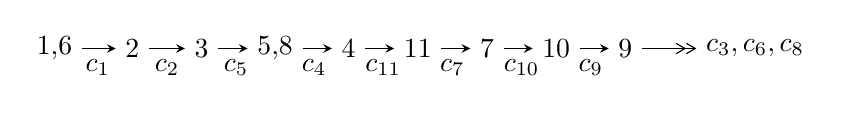
\begin{tikzpicture}[x=25pt, y=7pt]
	% node
	\node (A0) at (-1/8, 0) {1,6};
	\node (A1) at (1, 0) {2};
	\node (A2) at (2, 0) {3};
	\node (A3) at (49/16, 0) {5,8};
	\node (A4) at (33/8, 0) {4};
	\node (A5) at (41/8, 0) {11};
	\node (A6) at (49/8, 0) {7};
	\node (A7) at (57/8, 0) {10};
	\node (A8) at (65/8, 0) {9};
	\node (C1) at (1/2, -1) {$c_{1}$};
	\node (C2) at (3/2, -1) {$c_{2}$};
	\node (C3) at (5/2, -1) {$c_{5}$};
	\node (C4) at (29/8, -1) {$c_{4}$};
	\node (C5) at (37/8, -1) {$c_{11}$};
	\node (C6) at (45/8, -1) {$c_{7}$};
	\node (C7) at (53/8, -1) {$c_{10}$};
	\node (C8) at (61/8, -1) {$c_{9}$};
	\node (A9) at (10, 0) {$c_{3},c_{6},c_{8}$};

	% edge
	\draw[->,>=stealth]	
	(A0) edge (A1) (A1) edge (A2) (A2) edge (A3) (A3) edge (A4) (A4) edge (A5) (A5) edge (A6) (A6) edge (A7) (A7) edge (A8) ;
	\draw[->>,>={angle 60}]	
	(A8) edge (A9);
\end{tikzpicture} \\ 

\end{tabular} \\

\footnotetext{
The image of knot diagram is generated by the software ``\textbf{Draw programme}" developed by Andrew Bartholomew(\url{http://www.layer8.co.uk/maths/draw/index.htm\#Running-draw}), where we modified some parts for our purpose(\url{https://github.com/CATsTAILs/LinksPainter}).
}\phantom \\ \newline 
\centering \textbf{Ideals for irreducible components\footnotemark of $X_{\text{par}}$} 
 
\begin{align*}
I^u_{1}&=\langle 
-1238113 u^{25}+2413455 u^{24}+\cdots+2221939 b+1586090,\\
\phantom{I^u_{1}}&\phantom{= \langle  }4519597 u^{25}-816584 u^{24}+\cdots+13331634 a-13110217,\;u^{26}-2 u^{25}+\cdots- u+3\rangle \\
I^u_{2}&=\langle 
b-1,\;a^2-2 a u+2 a+u-2,\;u^2- u+1\rangle \\
I^u_{3}&=\langle 
b+1,\;a- u-1,\;u^2+u+1\rangle \\
\\
\end{align*}
\raggedright * 3 irreducible components of $\dim_{\mathbb{C}}=0$, with total 32 representations.\\
\footnotetext{All coefficients of polynomials are rational numbers. But the coefficients are sometimes approximated in decimal forms when there is not enough margin.}
\newpage
\renewcommand{\arraystretch}{1}
\centering \section*{I. $I^u_{1}= \langle -1.24\times10^{6} u^{25}+2.41\times10^{6} u^{24}+\cdots+2.22\times10^{6} b+1.59\times10^{6},\;4.52\times10^{6} u^{25}-8.17\times10^{5} u^{24}+\cdots+1.33\times10^{7} a-1.31\times10^{7},\;u^{26}-2 u^{25}+\cdots- u+3 \rangle$}
\flushleft \textbf{(i) Arc colorings}\\
\begin{tabular}{m{7pt} m{180pt} m{7pt} m{180pt} }
\flushright $a_{1}=$&$\begin{pmatrix}1\\0\end{pmatrix}$ \\
\flushright $a_{6}=$&$\begin{pmatrix}0\\u\end{pmatrix}$ \\
\flushright $a_{2}=$&$\begin{pmatrix}1\\- u^2\end{pmatrix}$ \\
\flushright $a_{3}=$&$\begin{pmatrix}u^2+1\\- u^2\end{pmatrix}$ \\
\flushright $a_{5}=$&$\begin{pmatrix}- u\\u^3+u\end{pmatrix}$ \\
\flushright $a_{8}=$&$\begin{pmatrix}-0.339013 u^{25}+0.0612516 u^{24}+\cdots+0.0332859 u+0.983392\\0.557222 u^{25}-1.08619 u^{24}+\cdots+1.41616 u-0.713831\end{pmatrix}$ \\
\flushright $a_{4}=$&$\begin{pmatrix}-0.254668 u^{25}+0.460389 u^{24}+\cdots-3.72725 u-2.65550\\0.0489476 u^{25}-0.702694 u^{24}+\cdots+2.91017 u-0.764005\end{pmatrix}$ \\
\flushright $a_{11}=$&$\begin{pmatrix}0.321877 u^{25}+0.0594569 u^{24}+\cdots-3.45009 u+0.683981\\-0.681651 u^{25}+1.22699 u^{24}+\cdots-0.0147380 u+0.770149\end{pmatrix}$ \\
\flushright $a_{7}=$&$\begin{pmatrix}- u^5-2 u^3- u\\u^5+u^3+u\end{pmatrix}$ \\
\flushright $a_{10}=$&$\begin{pmatrix}-0.359774 u^{25}+1.28645 u^{24}+\cdots-3.46483 u+1.45413\\-0.681651 u^{25}+1.22699 u^{24}+\cdots-0.0147380 u+0.770149\end{pmatrix}$ \\
\flushright $a_{9}=$&$\begin{pmatrix}0.237944 u^{25}+0.0813342 u^{24}+\cdots-2.32111 u+1.17821\\-0.616774 u^{25}+1.26410 u^{24}+\cdots+0.644379 u+1.01704\end{pmatrix}$\\ \flushright $a_{9}=$&$\begin{pmatrix}0.237944 u^{25}+0.0813342 u^{24}+\cdots-2.32111 u+1.17821\\-0.616774 u^{25}+1.26410 u^{24}+\cdots+0.644379 u+1.01704\end{pmatrix}$\\&\end{tabular}
\flushleft \textbf{(ii) Obstruction class $= -1$}\\~\\
\flushleft \textbf{(iii) Cusp Shapes $= -\frac{1151955}{2221939} u^{25}+\frac{814709}{2221939} u^{24}+\cdots-\frac{5153343}{2221939} u-\frac{28973115}{2221939}$}\\~\\
\newpage\renewcommand{\arraystretch}{1}
\flushleft \textbf{(iv) u-Polynomials at the component}\newline \\
\begin{tabular}{m{50pt}|m{274pt}}
Crossings & \hspace{64pt}u-Polynomials at each crossing \\
\hline $$\begin{aligned}c_{1},c_{5}\end{aligned}$$&$\begin{aligned}
&u^{26}-2 u^{25}+\cdots- u+3
\end{aligned}$\\
\hline $$\begin{aligned}c_{2}\end{aligned}$$&$\begin{aligned}
&u^{26}+16 u^{25}+\cdots-43 u+9
\end{aligned}$\\
\hline $$\begin{aligned}c_{3},c_{4},c_{8}\end{aligned}$$&$\begin{aligned}
&u^{26}+u^{25}+\cdots-8 u-4
\end{aligned}$\\
\hline $$\begin{aligned}c_{6}\end{aligned}$$&$\begin{aligned}
&u^{26}+2 u^{25}+\cdots-13 u+3
\end{aligned}$\\
\hline $$\begin{aligned}c_{7},c_{11}\end{aligned}$$&$\begin{aligned}
&u^{26}+3 u^{25}+\cdots+22 u-3
\end{aligned}$\\
\hline $$\begin{aligned}c_{9}\end{aligned}$$&$\begin{aligned}
&u^{26}- u^{25}+\cdots-32 u-4
\end{aligned}$\\
\hline $$\begin{aligned}c_{10}\end{aligned}$$&$\begin{aligned}
&u^{26}+33 u^{25}+\cdots+64 u+9
\end{aligned}$\\
\hline
\end{tabular}\\~\\
\newpage\renewcommand{\arraystretch}{1}
\flushleft \textbf{(v) Riley Polynomials at the component}\newline \\
\begin{tabular}{m{50pt}|m{274pt}}
Crossings & \hspace{64pt}Riley Polynomials at each crossing \\
\hline $$\begin{aligned}c_{1},c_{5}\end{aligned}$$&$\begin{aligned}
&y^{26}+16 y^{25}+\cdots-43 y+9
\end{aligned}$\\
\hline $$\begin{aligned}c_{2}\end{aligned}$$&$\begin{aligned}
&y^{26}-8 y^{25}+\cdots-7123 y+81
\end{aligned}$\\
\hline $$\begin{aligned}c_{3},c_{4},c_{8}\end{aligned}$$&$\begin{aligned}
&y^{26}+21 y^{25}+\cdots+64 y+16
\end{aligned}$\\
\hline $$\begin{aligned}c_{6}\end{aligned}$$&$\begin{aligned}
&y^{26}-32 y^{25}+\cdots-187 y+9
\end{aligned}$\\
\hline $$\begin{aligned}c_{7},c_{11}\end{aligned}$$&$\begin{aligned}
&y^{26}-33 y^{25}+\cdots-64 y+9
\end{aligned}$\\
\hline $$\begin{aligned}c_{9}\end{aligned}$$&$\begin{aligned}
&y^{26}-39 y^{25}+\cdots-128 y+16
\end{aligned}$\\
\hline $$\begin{aligned}c_{10}\end{aligned}$$&$\begin{aligned}
&y^{26}-73 y^{25}+\cdots+35108 y+81
\end{aligned}$\\
\hline
\end{tabular}\\~\\
\newpage\flushleft \textbf{(vi) Complex Volumes and Cusp Shapes}
$$\begin{array}{c|c|c}  
\text{Solutions to }I^u_{1}& \I (\text{vol} + \sqrt{-1}CS) & \text{Cusp shape}\\
 \hline 
\begin{aligned}
u &= \phantom{-}0.987320 + 0.168214 I \\
a &= \phantom{-}1.297460 + 0.513052 I \\
b &= -1.63497 - 0.20181 I\end{aligned}
 & -5.22414 - 5.39338 I & -6.45106 + 2.82273 I \\ \hline\begin{aligned}
u &= \phantom{-}0.987320 - 0.168214 I \\
a &= \phantom{-}1.297460 - 0.513052 I \\
b &= -1.63497 + 0.20181 I\end{aligned}
 & -5.22414 + 5.39338 I & -6.45106 - 2.82273 I \\ \hline\begin{aligned}
u &= -1.01037\phantom{ +0.000000I} \\
a &= -1.32902\phantom{ +0.000000I} \\
b &= \phantom{-}1.68442\phantom{ +0.000000I}\end{aligned}
 & -9.37437\phantom{ +0.000000I} & -9.45940\phantom{ +0.000000I} \\ \hline\begin{aligned}
u &= -0.541900 + 0.798242 I \\
a &= -1.229580 - 0.630085 I \\
b &= \phantom{-}0.190153 + 0.181187 I\end{aligned}
 & \phantom{-}4.95516 - 2.19764 I & \phantom{-}0.54342 + 3.86213 I \\ \hline\begin{aligned}
u &= -0.541900 - 0.798242 I \\
a &= -1.229580 + 0.630085 I \\
b &= \phantom{-}0.190153 - 0.181187 I\end{aligned}
 & \phantom{-}4.95516 + 2.19764 I & \phantom{-}0.54342 - 3.86213 I \\ \hline\begin{aligned}
u &= \phantom{-}0.280901 + 0.919746 I \\
a &= \phantom{-}0.066362 - 0.266060 I \\
b &= \phantom{-}0.270359 + 0.442643 I\end{aligned}
 & -0.60039 + 1.42912 I & -6.05587 - 3.68708 I \\ \hline\begin{aligned}
u &= \phantom{-}0.280901 - 0.919746 I \\
a &= \phantom{-}0.066362 + 0.266060 I \\
b &= \phantom{-}0.270359 - 0.442643 I\end{aligned}
 & -0.60039 - 1.42912 I & -6.05587 + 3.68708 I \\ \hline\begin{aligned}
u &= -0.086149 + 0.939073 I \\
a &= \phantom{-}1.12447 + 1.41361 I \\
b &= \phantom{-}1.170170 - 0.263604 I\end{aligned}
 & \phantom{-}1.87196 - 0.46648 I & -9.69334 - 0.39377 I \\ \hline\begin{aligned}
u &= -0.086149 - 0.939073 I \\
a &= \phantom{-}1.12447 - 1.41361 I \\
b &= \phantom{-}1.170170 + 0.263604 I\end{aligned}
 & \phantom{-}1.87196 + 0.46648 I & -9.69334 + 0.39377 I \\ \hline\begin{aligned}
u &= -0.714585 + 0.848170 I \\
a &= \phantom{-}1.111130 + 0.871548 I \\
b &= -1.336900 + 0.007719 I\end{aligned}
 & -0.16795 - 2.70526 I & -6.45261 + 3.54399 I\\
 \hline 
 \end{array}$$\newpage$$\begin{array}{c|c|c}  
\text{Solutions to }I^u_{1}& \I (\text{vol} + \sqrt{-1}CS) & \text{Cusp shape}\\
 \hline 
\begin{aligned}
u &= -0.714585 - 0.848170 I \\
a &= \phantom{-}1.111130 - 0.871548 I \\
b &= -1.336900 - 0.007719 I\end{aligned}
 & -0.16795 + 2.70526 I & -6.45261 - 3.54399 I \\ \hline\begin{aligned}
u &= \phantom{-}0.409972 + 1.042740 I \\
a &= -0.333921 + 0.008202 I \\
b &= \phantom{-}0.687191 + 0.474750 I\end{aligned}
 & -0.71901 + 1.35928 I & -6.71358 - 0.21049 I \\ \hline\begin{aligned}
u &= \phantom{-}0.409972 - 1.042740 I \\
a &= -0.333921 - 0.008202 I \\
b &= \phantom{-}0.687191 - 0.474750 I\end{aligned}
 & -0.71901 - 1.35928 I & -6.71358 + 0.21049 I \\ \hline\begin{aligned}
u &= -0.232752 + 1.110800 I \\
a &= -0.406380 + 1.143680 I \\
b &= -0.979109 - 0.571742 I\end{aligned}
 & -3.76323 - 2.26383 I & -13.05428 + 2.02208 I \\ \hline\begin{aligned}
u &= -0.232752 - 1.110800 I \\
a &= -0.406380 - 1.143680 I \\
b &= -0.979109 + 0.571742 I\end{aligned}
 & -3.76323 + 2.26383 I & -13.05428 - 2.02208 I \\ \hline\begin{aligned}
u &= \phantom{-}0.432711 + 1.187740 I \\
a &= \phantom{-}0.517506 + 1.268290 I \\
b &= \phantom{-}0.659883 - 0.866942 I\end{aligned}
 & -0.86443 + 6.41567 I & -7.45843 - 6.37638 I \\ \hline\begin{aligned}
u &= \phantom{-}0.432711 - 1.187740 I \\
a &= \phantom{-}0.517506 - 1.268290 I \\
b &= \phantom{-}0.659883 + 0.866942 I\end{aligned}
 & -0.86443 - 6.41567 I & -7.45843 + 6.37638 I \\ \hline\begin{aligned}
u &= \phantom{-}0.683039 + 0.071498 I \\
a &= -0.81507 - 1.50432 I \\
b &= \phantom{-}0.587913 + 0.647297 I\end{aligned}
 & \phantom{-}2.38839 - 2.21658 I & -3.00360 + 3.59199 I \\ \hline\begin{aligned}
u &= \phantom{-}0.683039 - 0.071498 I \\
a &= -0.81507 + 1.50432 I \\
b &= \phantom{-}0.587913 - 0.647297 I\end{aligned}
 & \phantom{-}2.38839 + 2.21658 I & -3.00360 - 3.59199 I \\ \hline\begin{aligned}
u &= \phantom{-}0.576371 + 1.269310 I \\
a &= -0.02214 - 1.67156 I \\
b &= -1.66528 + 0.31996 I\end{aligned}
 & -8.60064 + 11.02740 I & -8.81919 - 5.78425 I\\
 \hline 
 \end{array}$$\newpage$$\begin{array}{c|c|c}  
\text{Solutions to }I^u_{1}& \I (\text{vol} + \sqrt{-1}CS) & \text{Cusp shape}\\
 \hline 
\begin{aligned}
u &= \phantom{-}0.576371 - 1.269310 I \\
a &= -0.02214 + 1.67156 I \\
b &= -1.66528 - 0.31996 I\end{aligned}
 & -8.60064 - 11.02740 I & -8.81919 + 5.78425 I \\ \hline\begin{aligned}
u &= \phantom{-}0.376370 + 1.343310 I \\
a &= -0.157273 - 0.643532 I \\
b &= -1.74770 - 0.06929 I\end{aligned}
 & -10.10760 - 0.68348 I & -10.33009 + 0.33748 I \\ \hline\begin{aligned}
u &= \phantom{-}0.376370 - 1.343310 I \\
a &= -0.157273 + 0.643532 I \\
b &= -1.74770 + 0.06929 I\end{aligned}
 & -10.10760 + 0.68348 I & -10.33009 - 0.33748 I \\ \hline\begin{aligned}
u &= -0.49655 + 1.32834 I \\
a &= \phantom{-}0.015741 - 1.194450 I \\
b &= \phantom{-}1.76275 + 0.15335 I\end{aligned}
 & -13.5263 - 5.3591 I & -12.04516 + 3.16064 I \\ \hline\begin{aligned}
u &= -0.49655 - 1.32834 I \\
a &= \phantom{-}0.015741 + 1.194450 I \\
b &= \phantom{-}1.76275 - 0.15335 I\end{aligned}
 & -13.5263 + 5.3591 I & -12.04516 - 3.16064 I \\ \hline\begin{aligned}
u &= -0.339124\phantom{ +0.000000I} \\
a &= \phantom{-}1.65907\phantom{ +0.000000I} \\
b &= -0.613341\phantom{ +0.000000I}\end{aligned}
 & -0.865956\phantom{ +0.000000I} & -11.4730\phantom{ +0.000000I}\\
 \hline 
 \end{array}$$\newpage\newpage\renewcommand{\arraystretch}{1}
\centering \section*{II. $I^u_{2}= \langle b-1,\;a^2-2 a u+2 a+u-2,\;u^2- u+1 \rangle$}
\flushleft \textbf{(i) Arc colorings}\\
\begin{tabular}{m{7pt} m{180pt} m{7pt} m{180pt} }
\flushright $a_{1}=$&$\begin{pmatrix}1\\0\end{pmatrix}$ \\
\flushright $a_{6}=$&$\begin{pmatrix}0\\u\end{pmatrix}$ \\
\flushright $a_{2}=$&$\begin{pmatrix}1\\- u+1\end{pmatrix}$ \\
\flushright $a_{3}=$&$\begin{pmatrix}u\\- u+1\end{pmatrix}$ \\
\flushright $a_{5}=$&$\begin{pmatrix}- u\\u-1\end{pmatrix}$ \\
\flushright $a_{8}=$&$\begin{pmatrix}a\\1\end{pmatrix}$ \\
\flushright $a_{4}=$&$\begin{pmatrix}- a u+u-1\\a u- a+2 u-1\end{pmatrix}$ \\
\flushright $a_{11}=$&$\begin{pmatrix}- a+1\\-1\end{pmatrix}$ \\
\flushright $a_{7}=$&$\begin{pmatrix}1\\0\end{pmatrix}$ \\
\flushright $a_{10}=$&$\begin{pmatrix}- a\\-1\end{pmatrix}$ \\
\flushright $a_{9}=$&$\begin{pmatrix}- u+1\\- a u-2\end{pmatrix}$\\ \flushright $a_{9}=$&$\begin{pmatrix}- u+1\\- a u-2\end{pmatrix}$\\&\end{tabular}
\flushleft \textbf{(ii) Obstruction class $= 1$}\\~\\
\flushleft \textbf{(iii) Cusp Shapes $= -4 u-4$}\\~\\
\newpage\renewcommand{\arraystretch}{1}
\flushleft \textbf{(iv) u-Polynomials at the component}\newline \\
\begin{tabular}{m{50pt}|m{274pt}}
Crossings & \hspace{64pt}u-Polynomials at each crossing \\
\hline $$\begin{aligned}c_{1},c_{6}\end{aligned}$$&$\begin{aligned}
&(u^2- u+1)^2
\end{aligned}$\\
\hline $$\begin{aligned}c_{2},c_{5}\end{aligned}$$&$\begin{aligned}
&(u^2+u+1)^2
\end{aligned}$\\
\hline $$\begin{aligned}c_{3},c_{4},c_{8}\\c_{9}\end{aligned}$$&$\begin{aligned}
&(u^2+2)^2
\end{aligned}$\\
\hline $$\begin{aligned}c_{7}\end{aligned}$$&$\begin{aligned}
&(u+1)^4
\end{aligned}$\\
\hline $$\begin{aligned}c_{10},c_{11}\end{aligned}$$&$\begin{aligned}
&(u-1)^4
\end{aligned}$\\
\hline
\end{tabular}\\~\\
\newpage\renewcommand{\arraystretch}{1}
\flushleft \textbf{(v) Riley Polynomials at the component}\newline \\
\begin{tabular}{m{50pt}|m{274pt}}
Crossings & \hspace{64pt}Riley Polynomials at each crossing \\
\hline $$\begin{aligned}c_{1},c_{2},c_{5}\\c_{6}\end{aligned}$$&$\begin{aligned}
&(y^2+y+1)^2
\end{aligned}$\\
\hline $$\begin{aligned}c_{3},c_{4},c_{8}\\c_{9}\end{aligned}$$&$\begin{aligned}
&(y+2)^4
\end{aligned}$\\
\hline $$\begin{aligned}c_{7},c_{10},c_{11}\end{aligned}$$&$\begin{aligned}
&(y-1)^4
\end{aligned}$\\
\hline
\end{tabular}\\~\\
\newpage\flushleft \textbf{(vi) Complex Volumes and Cusp Shapes}
$$\begin{array}{c|c|c}  
\text{Solutions to }I^u_{2}& \I (\text{vol} + \sqrt{-1}CS) & \text{Cusp shape}\\
 \hline 
\begin{aligned}
u &= \phantom{-}0.500000 + 0.866025 I \\
a &= \phantom{-}0.724745 + 0.158919 I \\
b &= \phantom{-}1.00000\phantom{ +0.000000I}\end{aligned}
 & \phantom{-}3.28987 + 2.02988 I & -6.00000 - 3.46410 I \\ \hline\begin{aligned}
u &= \phantom{-}0.500000 + 0.866025 I \\
a &= -1.72474 + 1.57313 I \\
b &= \phantom{-}1.00000\phantom{ +0.000000I}\end{aligned}
 & \phantom{-}3.28987 + 2.02988 I & -6.00000 - 3.46410 I \\ \hline\begin{aligned}
u &= \phantom{-}0.500000 - 0.866025 I \\
a &= \phantom{-}0.724745 - 0.158919 I \\
b &= \phantom{-}1.00000\phantom{ +0.000000I}\end{aligned}
 & \phantom{-}3.28987 - 2.02988 I & -6.00000 + 3.46410 I \\ \hline\begin{aligned}
u &= \phantom{-}0.500000 - 0.866025 I \\
a &= -1.72474 - 1.57313 I \\
b &= \phantom{-}1.00000\phantom{ +0.000000I}\end{aligned}
 & \phantom{-}3.28987 - 2.02988 I & -6.00000 + 3.46410 I\\
 \hline 
 \end{array}$$\newpage\newpage\renewcommand{\arraystretch}{1}
\centering \section*{III. $I^u_{3}= \langle b+1,\;a- u-1,\;u^2+u+1 \rangle$}
\flushleft \textbf{(i) Arc colorings}\\
\begin{tabular}{m{7pt} m{180pt} m{7pt} m{180pt} }
\flushright $a_{1}=$&$\begin{pmatrix}1\\0\end{pmatrix}$ \\
\flushright $a_{6}=$&$\begin{pmatrix}0\\u\end{pmatrix}$ \\
\flushright $a_{2}=$&$\begin{pmatrix}1\\u+1\end{pmatrix}$ \\
\flushright $a_{3}=$&$\begin{pmatrix}- u\\u+1\end{pmatrix}$ \\
\flushright $a_{5}=$&$\begin{pmatrix}- u\\u+1\end{pmatrix}$ \\
\flushright $a_{8}=$&$\begin{pmatrix}u+1\\-1\end{pmatrix}$ \\
\flushright $a_{4}=$&$\begin{pmatrix}- u\\u+1\end{pmatrix}$ \\
\flushright $a_{11}=$&$\begin{pmatrix}u+2\\-1\end{pmatrix}$ \\
\flushright $a_{7}=$&$\begin{pmatrix}-1\\0\end{pmatrix}$ \\
\flushright $a_{10}=$&$\begin{pmatrix}u+1\\-1\end{pmatrix}$ \\
\flushright $a_{9}=$&$\begin{pmatrix}u+1\\-1\end{pmatrix}$\\ \flushright $a_{9}=$&$\begin{pmatrix}u+1\\-1\end{pmatrix}$\\&\end{tabular}
\flushleft \textbf{(ii) Obstruction class $= 1$}\\~\\
\flushleft \textbf{(iii) Cusp Shapes $= 4 u-10$}\\~\\
\newpage\renewcommand{\arraystretch}{1}
\flushleft \textbf{(iv) u-Polynomials at the component}\newline \\
\begin{tabular}{m{50pt}|m{274pt}}
Crossings & \hspace{64pt}u-Polynomials at each crossing \\
\hline $$\begin{aligned}c_{1},c_{2},c_{6}\end{aligned}$$&$\begin{aligned}
&u^2+u+1
\end{aligned}$\\
\hline $$\begin{aligned}c_{3},c_{4},c_{8}\\c_{9}\end{aligned}$$&$\begin{aligned}
&u^2
\end{aligned}$\\
\hline $$\begin{aligned}c_{5}\end{aligned}$$&$\begin{aligned}
&u^2- u+1
\end{aligned}$\\
\hline $$\begin{aligned}c_{7},c_{10}\end{aligned}$$&$\begin{aligned}
&(u-1)^2
\end{aligned}$\\
\hline $$\begin{aligned}c_{11}\end{aligned}$$&$\begin{aligned}
&(u+1)^2
\end{aligned}$\\
\hline
\end{tabular}\\~\\
\newpage\renewcommand{\arraystretch}{1}
\flushleft \textbf{(v) Riley Polynomials at the component}\newline \\
\begin{tabular}{m{50pt}|m{274pt}}
Crossings & \hspace{64pt}Riley Polynomials at each crossing \\
\hline $$\begin{aligned}c_{1},c_{2},c_{5}\\c_{6}\end{aligned}$$&$\begin{aligned}
&y^2+y+1
\end{aligned}$\\
\hline $$\begin{aligned}c_{3},c_{4},c_{8}\\c_{9}\end{aligned}$$&$\begin{aligned}
&y^2
\end{aligned}$\\
\hline $$\begin{aligned}c_{7},c_{10},c_{11}\end{aligned}$$&$\begin{aligned}
&(y-1)^2
\end{aligned}$\\
\hline
\end{tabular}\\~\\
\newpage\flushleft \textbf{(vi) Complex Volumes and Cusp Shapes}
$$\begin{array}{c|c|c}  
\text{Solutions to }I^u_{3}& \I (\text{vol} + \sqrt{-1}CS) & \text{Cusp shape}\\
 \hline 
\begin{aligned}
u &= -0.500000 + 0.866025 I \\
a &= \phantom{-}0.500000 + 0.866025 I \\
b &= -1.00000\phantom{ +0.000000I}\end{aligned}
 & -1.64493 - 2.02988 I & -12.00000 + 3.46410 I \\ \hline\begin{aligned}
u &= -0.500000 - 0.866025 I \\
a &= \phantom{-}0.500000 - 0.866025 I \\
b &= -1.00000\phantom{ +0.000000I}\end{aligned}
 & -1.64493 + 2.02988 I & -12.00000 - 3.46410 I\\
 \hline 
 \end{array}$$\newpage
\newpage\renewcommand{\arraystretch}{1}
\centering \section*{ IV. u-Polynomials}
\begin{tabular}{m{50pt}|m{274pt}}
Crossings & \hspace{64pt}u-Polynomials at each crossing \\
\hline $$\begin{aligned}c_{1}\end{aligned}$$&$\begin{aligned}
&((u^2- u+1)^2)(u^2+u+1)(u^{26}-2 u^{25}+\cdots- u+3)
\end{aligned}$\\
\hline $$\begin{aligned}c_{2}\end{aligned}$$&$\begin{aligned}
&((u^2+u+1)^3)(u^{26}+16 u^{25}+\cdots-43 u+9)
\end{aligned}$\\
\hline $$\begin{aligned}c_{3},c_{4},c_{8}\end{aligned}$$&$\begin{aligned}
&u^2(u^2+2)^2(u^{26}+u^{25}+\cdots-8 u-4)
\end{aligned}$\\
\hline $$\begin{aligned}c_{5}\end{aligned}$$&$\begin{aligned}
&(u^2- u+1)(u^2+u+1)^2(u^{26}-2 u^{25}+\cdots- u+3)
\end{aligned}$\\
\hline $$\begin{aligned}c_{6}\end{aligned}$$&$\begin{aligned}
&((u^2- u+1)^2)(u^2+u+1)(u^{26}+2 u^{25}+\cdots-13 u+3)
\end{aligned}$\\
\hline $$\begin{aligned}c_{7}\end{aligned}$$&$\begin{aligned}
&((u-1)^2)(u+1)^4(u^{26}+3 u^{25}+\cdots+22 u-3)
\end{aligned}$\\
\hline $$\begin{aligned}c_{9}\end{aligned}$$&$\begin{aligned}
&u^2(u^2+2)^2(u^{26}- u^{25}+\cdots-32 u-4)
\end{aligned}$\\
\hline $$\begin{aligned}c_{10}\end{aligned}$$&$\begin{aligned}
&((u-1)^6)(u^{26}+33 u^{25}+\cdots+64 u+9)
\end{aligned}$\\
\hline $$\begin{aligned}c_{11}\end{aligned}$$&$\begin{aligned}
&((u-1)^4)(u+1)^2(u^{26}+3 u^{25}+\cdots+22 u-3)
\end{aligned}$\\
\hline
\end{tabular}\newpage\renewcommand{\arraystretch}{1}
\centering \section*{ V. Riley Polynomials}
\begin{tabular}{m{50pt}|m{274pt}}
Crossings & \hspace{64pt}Riley Polynomials at each crossing \\
\hline $$\begin{aligned}c_{1},c_{5}\end{aligned}$$&$\begin{aligned}
&((y^2+y+1)^3)(y^{26}+16 y^{25}+\cdots-43 y+9)
\end{aligned}$\\
\hline $$\begin{aligned}c_{2}\end{aligned}$$&$\begin{aligned}
&((y^2+y+1)^3)(y^{26}-8 y^{25}+\cdots-7123 y+81)
\end{aligned}$\\
\hline $$\begin{aligned}c_{3},c_{4},c_{8}\end{aligned}$$&$\begin{aligned}
&y^2(y+2)^4(y^{26}+21 y^{25}+\cdots+64 y+16)
\end{aligned}$\\
\hline $$\begin{aligned}c_{6}\end{aligned}$$&$\begin{aligned}
&((y^2+y+1)^3)(y^{26}-32 y^{25}+\cdots-187 y+9)
\end{aligned}$\\
\hline $$\begin{aligned}c_{7},c_{11}\end{aligned}$$&$\begin{aligned}
&((y-1)^6)(y^{26}-33 y^{25}+\cdots-64 y+9)
\end{aligned}$\\
\hline $$\begin{aligned}c_{9}\end{aligned}$$&$\begin{aligned}
&y^2(y+2)^4(y^{26}-39 y^{25}+\cdots-128 y+16)
\end{aligned}$\\
\hline $$\begin{aligned}c_{10}\end{aligned}$$&$\begin{aligned}
&((y-1)^6)(y^{26}-73 y^{25}+\cdots+35108 y+81)
\end{aligned}$\\
\hline
\end{tabular}
\vskip 2pc
\end{document}